\documentclass[]{book}
\usepackage{lmodern}
\usepackage{amssymb,amsmath}
\usepackage{ifxetex,ifluatex}
\usepackage{fixltx2e} % provides \textsubscript
\ifnum 0\ifxetex 1\fi\ifluatex 1\fi=0 % if pdftex
  \usepackage[T1]{fontenc}
  \usepackage[utf8]{inputenc}
\else % if luatex or xelatex
  \ifxetex
    \usepackage{mathspec}
  \else
    \usepackage{fontspec}
  \fi
  \defaultfontfeatures{Ligatures=TeX,Scale=MatchLowercase}
\fi
% use upquote if available, for straight quotes in verbatim environments
\IfFileExists{upquote.sty}{\usepackage{upquote}}{}
% use microtype if available
\IfFileExists{microtype.sty}{%
\usepackage[]{microtype}
\UseMicrotypeSet[protrusion]{basicmath} % disable protrusion for tt fonts
}{}
\PassOptionsToPackage{hyphens}{url} % url is loaded by hyperref
\usepackage[unicode=true]{hyperref}
\hypersetup{
            pdftitle={Datenanalyse: Eye-tracking 2020/2021},
            pdfauthor={Katja Suckow},
            pdfborder={0 0 0},
            breaklinks=true}
\urlstyle{same}  % don't use monospace font for urls
\usepackage{natbib}
\bibliographystyle{apalike}
\usepackage{color}
\usepackage{fancyvrb}
\newcommand{\VerbBar}{|}
\newcommand{\VERB}{\Verb[commandchars=\\\{\}]}
\DefineVerbatimEnvironment{Highlighting}{Verbatim}{commandchars=\\\{\}}
% Add ',fontsize=\small' for more characters per line
\usepackage{framed}
\definecolor{shadecolor}{RGB}{248,248,248}
\newenvironment{Shaded}{\begin{snugshade}}{\end{snugshade}}
\newcommand{\KeywordTok}[1]{\textcolor[rgb]{0.13,0.29,0.53}{\textbf{#1}}}
\newcommand{\DataTypeTok}[1]{\textcolor[rgb]{0.13,0.29,0.53}{#1}}
\newcommand{\DecValTok}[1]{\textcolor[rgb]{0.00,0.00,0.81}{#1}}
\newcommand{\BaseNTok}[1]{\textcolor[rgb]{0.00,0.00,0.81}{#1}}
\newcommand{\FloatTok}[1]{\textcolor[rgb]{0.00,0.00,0.81}{#1}}
\newcommand{\ConstantTok}[1]{\textcolor[rgb]{0.00,0.00,0.00}{#1}}
\newcommand{\CharTok}[1]{\textcolor[rgb]{0.31,0.60,0.02}{#1}}
\newcommand{\SpecialCharTok}[1]{\textcolor[rgb]{0.00,0.00,0.00}{#1}}
\newcommand{\StringTok}[1]{\textcolor[rgb]{0.31,0.60,0.02}{#1}}
\newcommand{\VerbatimStringTok}[1]{\textcolor[rgb]{0.31,0.60,0.02}{#1}}
\newcommand{\SpecialStringTok}[1]{\textcolor[rgb]{0.31,0.60,0.02}{#1}}
\newcommand{\ImportTok}[1]{#1}
\newcommand{\CommentTok}[1]{\textcolor[rgb]{0.56,0.35,0.01}{\textit{#1}}}
\newcommand{\DocumentationTok}[1]{\textcolor[rgb]{0.56,0.35,0.01}{\textbf{\textit{#1}}}}
\newcommand{\AnnotationTok}[1]{\textcolor[rgb]{0.56,0.35,0.01}{\textbf{\textit{#1}}}}
\newcommand{\CommentVarTok}[1]{\textcolor[rgb]{0.56,0.35,0.01}{\textbf{\textit{#1}}}}
\newcommand{\OtherTok}[1]{\textcolor[rgb]{0.56,0.35,0.01}{#1}}
\newcommand{\FunctionTok}[1]{\textcolor[rgb]{0.00,0.00,0.00}{#1}}
\newcommand{\VariableTok}[1]{\textcolor[rgb]{0.00,0.00,0.00}{#1}}
\newcommand{\ControlFlowTok}[1]{\textcolor[rgb]{0.13,0.29,0.53}{\textbf{#1}}}
\newcommand{\OperatorTok}[1]{\textcolor[rgb]{0.81,0.36,0.00}{\textbf{#1}}}
\newcommand{\BuiltInTok}[1]{#1}
\newcommand{\ExtensionTok}[1]{#1}
\newcommand{\PreprocessorTok}[1]{\textcolor[rgb]{0.56,0.35,0.01}{\textit{#1}}}
\newcommand{\AttributeTok}[1]{\textcolor[rgb]{0.77,0.63,0.00}{#1}}
\newcommand{\RegionMarkerTok}[1]{#1}
\newcommand{\InformationTok}[1]{\textcolor[rgb]{0.56,0.35,0.01}{\textbf{\textit{#1}}}}
\newcommand{\WarningTok}[1]{\textcolor[rgb]{0.56,0.35,0.01}{\textbf{\textit{#1}}}}
\newcommand{\AlertTok}[1]{\textcolor[rgb]{0.94,0.16,0.16}{#1}}
\newcommand{\ErrorTok}[1]{\textcolor[rgb]{0.64,0.00,0.00}{\textbf{#1}}}
\newcommand{\NormalTok}[1]{#1}
\usepackage{longtable,booktabs}
% Fix footnotes in tables (requires footnote package)
\IfFileExists{footnote.sty}{\usepackage{footnote}\makesavenoteenv{long table}}{}
\usepackage{graphicx,grffile}
\makeatletter
\def\maxwidth{\ifdim\Gin@nat@width>\linewidth\linewidth\else\Gin@nat@width\fi}
\def\maxheight{\ifdim\Gin@nat@height>\textheight\textheight\else\Gin@nat@height\fi}
\makeatother
% Scale images if necessary, so that they will not overflow the page
% margins by default, and it is still possible to overwrite the defaults
% using explicit options in \includegraphics[width, height, ...]{}
\setkeys{Gin}{width=\maxwidth,height=\maxheight,keepaspectratio}
\IfFileExists{parskip.sty}{%
\usepackage{parskip}
}{% else
\setlength{\parindent}{0pt}
\setlength{\parskip}{6pt plus 2pt minus 1pt}
}
\setlength{\emergencystretch}{3em}  % prevent overfull lines
\providecommand{\tightlist}{%
  \setlength{\itemsep}{0pt}\setlength{\parskip}{0pt}}
\setcounter{secnumdepth}{5}
% Redefines (sub)paragraphs to behave more like sections
\ifx\paragraph\undefined\else
\let\oldparagraph\paragraph
\renewcommand{\paragraph}[1]{\oldparagraph{#1}\mbox{}}
\fi
\ifx\subparagraph\undefined\else
\let\oldsubparagraph\subparagraph
\renewcommand{\subparagraph}[1]{\oldsubparagraph{#1}\mbox{}}
\fi

% set default figure placement to htbp
\makeatletter
\def\fps@figure{htbp}
\makeatother

\usepackage{booktabs}

\title{Datenanalyse: Eye-tracking 2020/2021}
\author{Katja Suckow}
\date{2021-01-22}

\begin{document}
\maketitle

{
\setcounter{tocdepth}{1}
\tableofcontents
}
\chapter{Willkommen}\label{willkommen}

Da wir uns leider in diesem Jahr erstmal nicht persönlich treffen
können, habe ich hier eine kleine Übersicht zu den verwendeten
R-Befehlen erstellt.

\section{Was braucht man dafür?}\label{was-braucht-man-dafuxfcr}

Dafür muss man auf seinem Rechner \textbf{R} und \textbf{Rstudio}
installieren (beide sollten auf Windows, Mac und Linux laufen).

\begin{enumerate}
\def\labelenumi{\arabic{enumi}.}
\tightlist
\item
  \textbf{R} frei verfügbare Software \url{https://www.r-project.org/}
\end{enumerate}

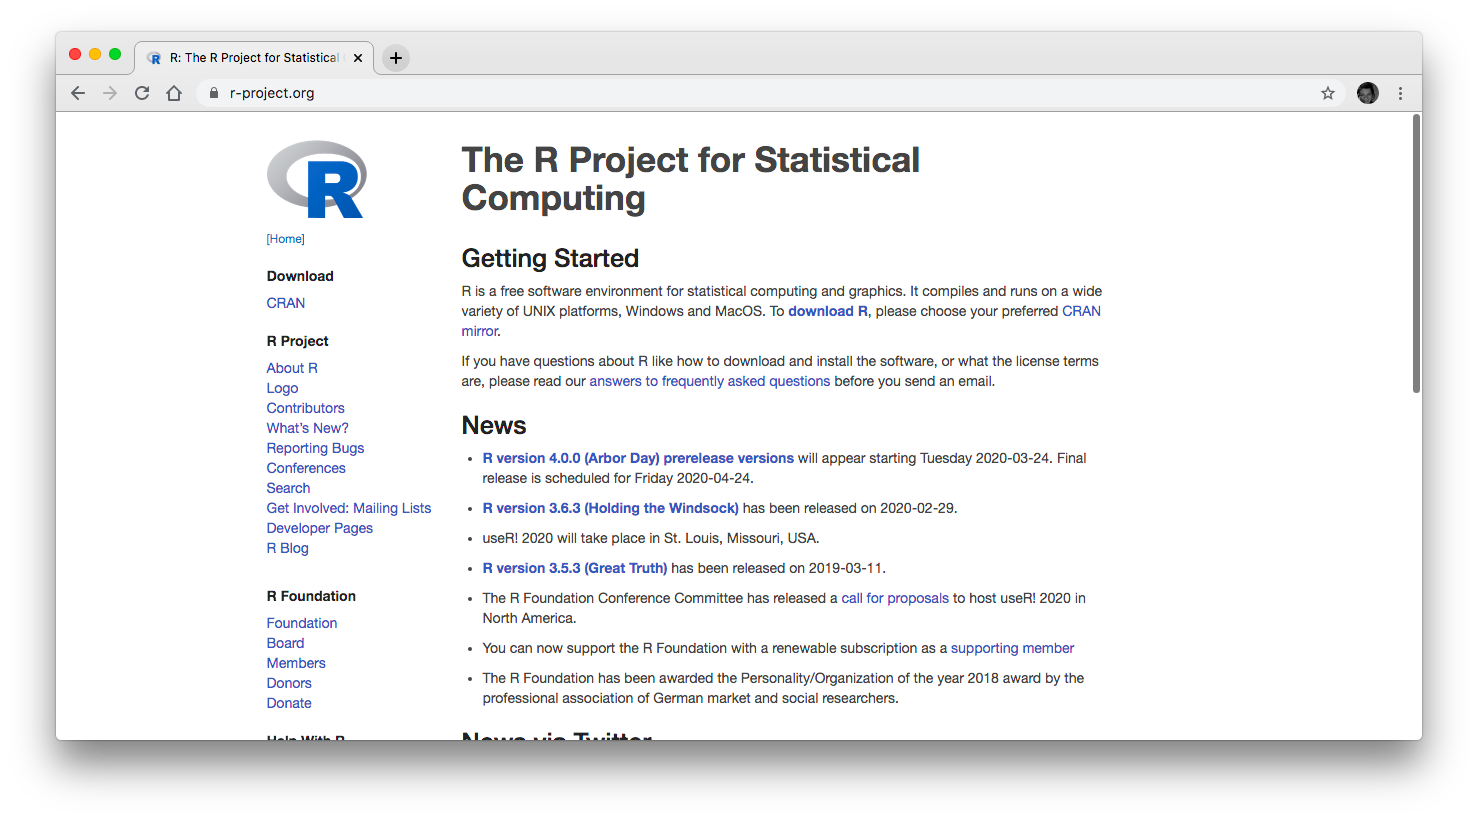
\includegraphics{./img/Rdownload.png} \textbf{R} ist eine freie
Programmiersprache zur statistischen Datenanalyse und Erstellung von
Grafiken. Sie kann auch als Skriptsprache benutzt werden, um einfache
Skripte und Programme zu schreiben. \textbf{R} ist vor allem in der
Wissenschaft weit verbreitet und löst hier zunehmend SPSS ab. \textbf{R}
bietet viele Methoden und Pakete zu statistischen Auswertung und
Datendarstellung, die ständig in open-source weiterentwickelt werden, es
steht kostenlos zur Verfügung und kann auf jeder Plattform (Windows,
Mac, Linux) laufen. R besteht aus 3 Hauptfenstern: (1) \textbf{Konsole},
um direkt Befehle einzugeben, (2) \textbf{Editor}, um eine Abfolge an
Befehlen zu speichern und auszuführen, (3) \textbf{Grafikfenster}

\begin{enumerate}
\def\labelenumi{\arabic{enumi}.}
\setcounter{enumi}{1}
\tightlist
\item
  \textbf{RStudio}
  \url{https://www.rstudio.com/products/rstudio/download} Es gibt
  verschiedene Möglichkeiten mit R zu arbeiten. Wir werden die grafische
  Oberfläche, die \textbf{RStudio} bietet, nutzen. \textbf{RStudio}
  bietet eine gut handhabe Oberfläche, viel Unterstützung und viele
  integrierte Apps (Shiny, Markdown, Bookdown \ldots{}), die auf R
  zurückgreifen. Unterschiedliche Editoren zur Bearbeitung von R Dateien
  sind:
\end{enumerate}

\begin{itemize}
\tightlist
\item
  RStudio (für die gemeinsame Datenauswertung im Praktikum empfohlen)
\item
  Notepad++ (Windows)
\item
  Textwrangler
\item
  \(\dots\)
\end{itemize}

\begin{figure}
\centering

\includegraphics{./img/download.jpg}
\caption{RStudio Logo}
\end{figure}

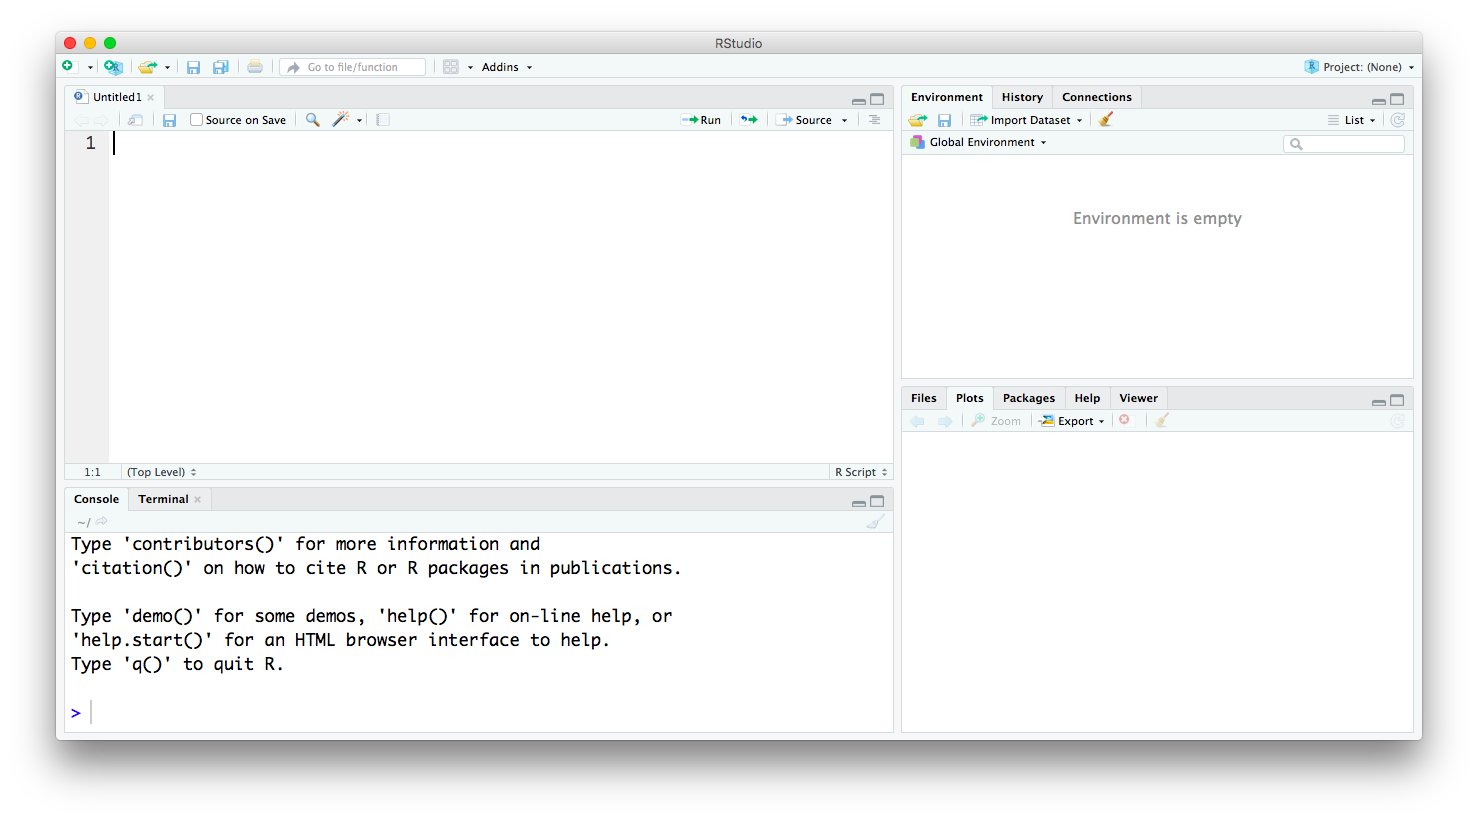
\includegraphics{./img/RStudio-look1.png} So sieht RStudio ohne Inhalt
oder Daten aus.

\begin{figure}
\centering
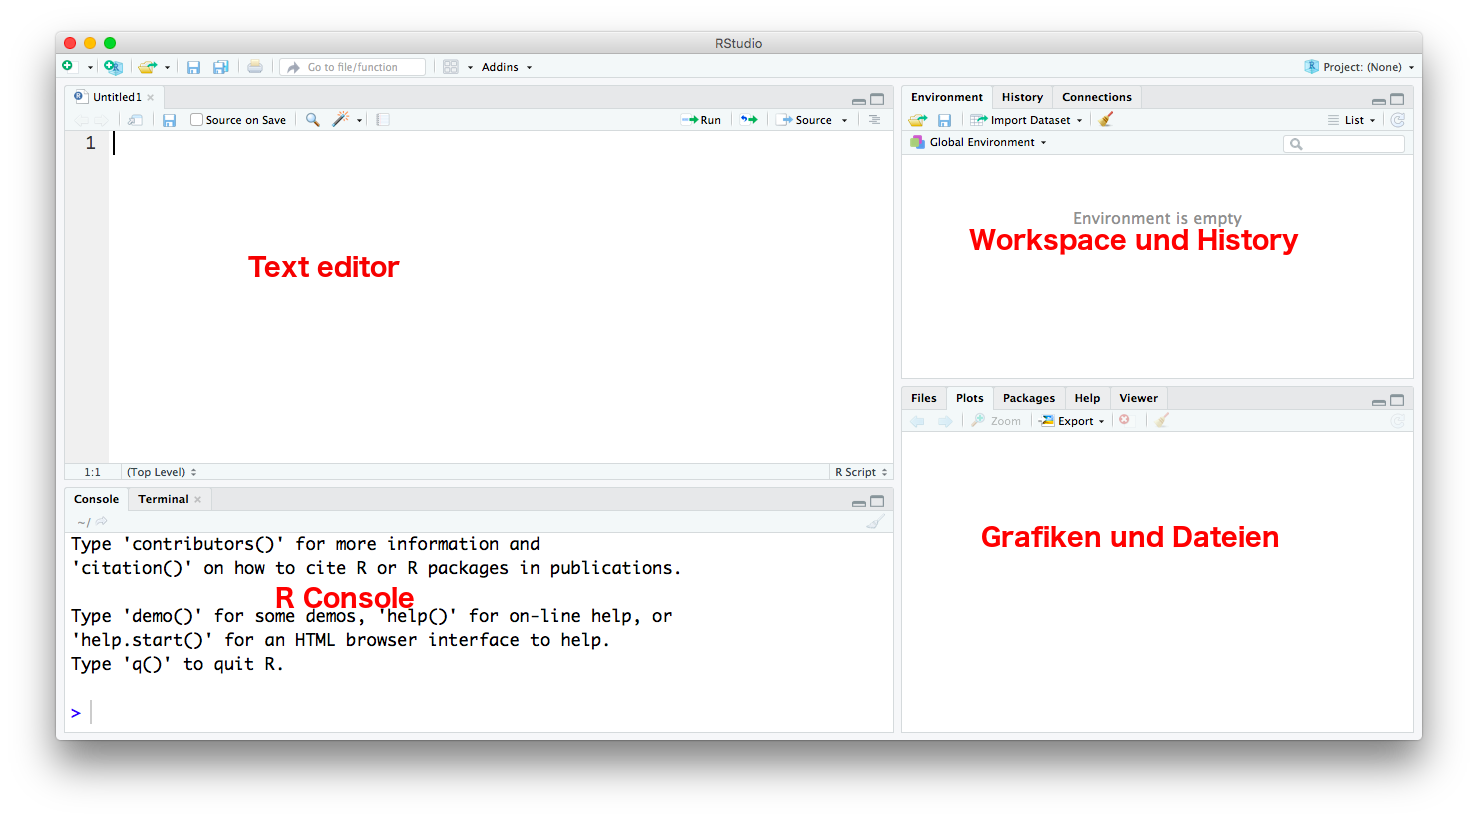
\includegraphics{./img/RStudio-look.png}
\caption{Die 4 Hauptfenster von RStudio}
\end{figure}

In der Standarddarstellung befindet sich oben links der \textbf{Code
Editor}, oben rechts können sie \textbf{Workspace und History} ansehen,
unten links befindet sich die \textbf{R Console}, in der Sie den Code
direkt eingeben können und unten rechts lassen sich unter anderem
\textbf{Plots und Files} anzeigen. Schauen Sie sich die verschiedenen
Möglichkeiten an, die die verschiedenen Tabs in den Ecken bieten.

\textbf{Skript}

Das Skript enthält eine Sammlung von Befehlen. Diese können auch direkt
über Konsole ausgeführt werden. Es empfiehlt sich jedoch sehr, diese im
\textbf{Code Editor} zu speichern, um später noch einmal darauf
zugreifen zu können.

\textbf{Workspace}

Der Workspace enthält Sammlung von Objekten, die in einer Session
erstellt wurden. Diese kann explizit gespeichert werden, um die
einzelnen Objekte noch einmal neu zu laden.

So sieht Rstudio mit ein bischen mehr Inhalt aus.

\begin{figure}
\centering
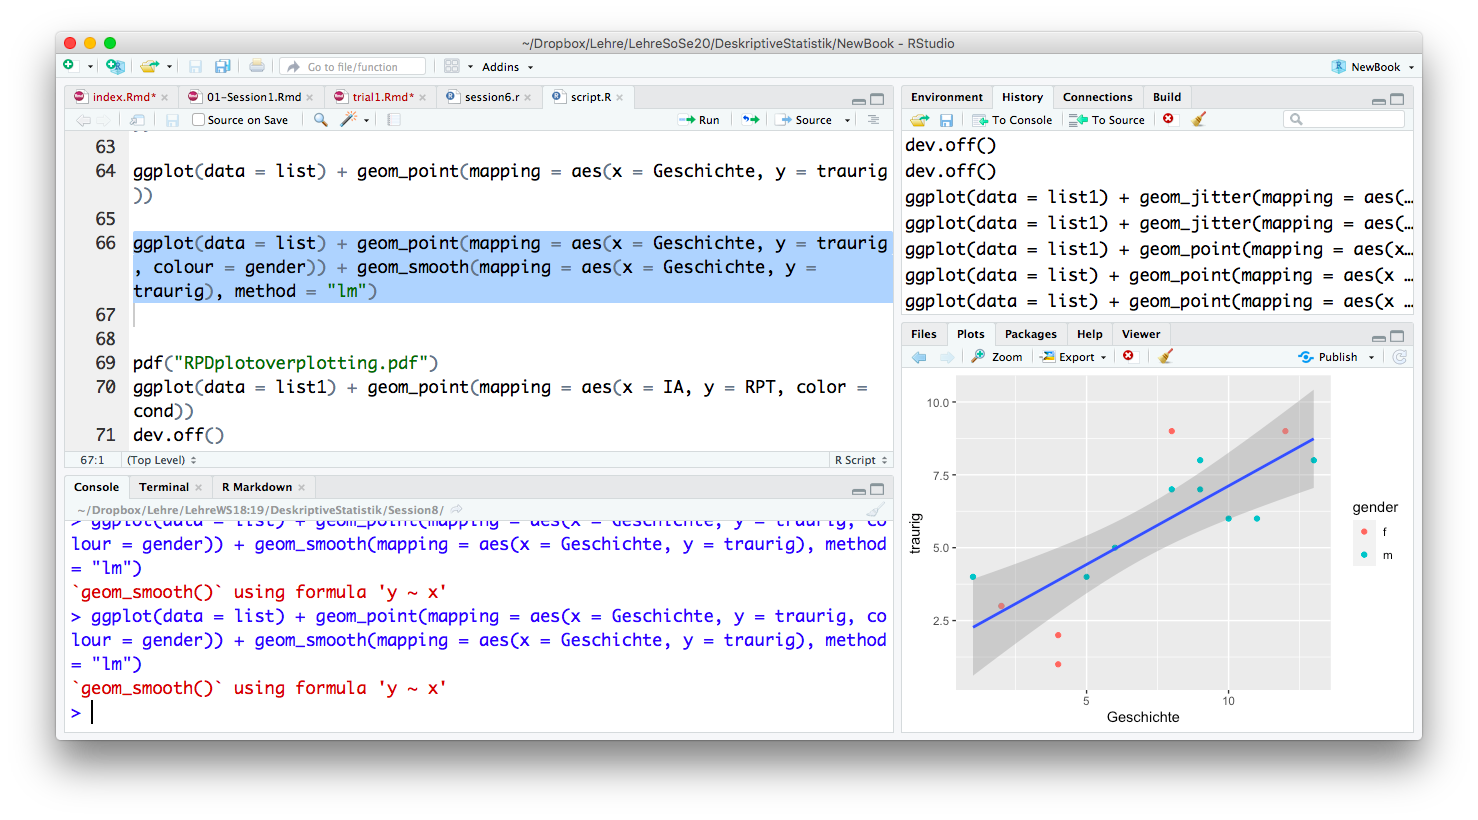
\includegraphics{./img/ScreenGrafik.png}
\caption{RStudio mit Datensatz und grafischer Darstellung eines
Datensatzes}
\end{figure}

\begin{itemize}
\tightlist
\item
  \textbf{oben links} steht der Code, der gespeichert und auch aus dem
  Editor ausgeführt werden kann. (Mac: Markierung des auszuführenden
  Codes und dann \textbf{CMD + Enter})
\item
  \textbf{unten links} man kannn den auszuführenden Code auch direkt
  unten in das Konsolenfenster eingeben. Dann wird dieser allerdings
  nicht gespeichert. Es wird empfohlen, Code der erstmal nur ausprobiert
  wird, direkt in das Konsolenfenster einzutragen. Wenn der Code das
  korrekte Ergebnis liefert, sollte er im Editor in einem Skript
  gespeichert werden.
\item
  \textbf{oben rechts} lassen sich History der eingegebenen Befehle und
  auch die Inhalte des Workspace anzeigen
\item
  \textbf{unten rechts} kann man sich die geladenen Pakete für
  \textbf{R}, sowie die verschiedenen erstellten Grafiken anzeigen
  lassen
\end{itemize}

Die Anordnung der Fenster lassen sich über \textbf{RStudio}
\textgreater{} \textbf{Preferences} und dann \textbf{Pane Layout}
ändern. Über \textbf{Preferences} können Sie sich generell anzeigen
lassen, welche Änderungen Sie u.a. bei der Anzeige vornehmen können
bzw.\textasciitilde{}wollen.

\section{Einleitung: Datentypen in der
Linguistik}\label{einleitung-datentypen-in-der-linguistik}

\textbf{Qualitative Daten} Nicht-numerische, oft verschriftlichte oder
in audiovisueller Form vorliegende Daten. Verwendung häufig explorativ
und hypothesengenerierend. (e.g., Interviews)

\textbf{Quantitative Daten} Numerische (bzw. in numerischer Form
überführte) Daten, die mit dem Ziel der Überprüfung von Hypothesen und
Theorien erhoben werden

\section{Population und Stichprobe}\label{population-und-stichprobe}

In der psycholinguistischen Forschung werden Daten in einer
kontrollierten Umgebung (Experiment) erhoben, die Aussagen für die
Gesamtpopulation zu einer bestimmten linguistischen Fragestellung machen
zu können.

Dabei wird eine kleine Gruppe der Population (Stichprobe) in einem
Experiment getestet. Bestimmte Daten dieser Stichprobe werden erhoben
und anschliessend die Ergebnisse dieser Daten auf die Gesamtpopulation
projiziert. Die erhobenen Daten der Stichprobe müssen erst in
deskriptive statistische Kennwerte umgewandelt werden und anschliessend
mittels statistischer Verfahren Hypothesen geprüft werden, um Aussagen
über die Gesamtpopulation machen zu können.

\section{Deskriptive Statistik und
Inferenzstatistik}\label{deskriptive-statistik-und-inferenzstatistik}

\textbf{Deskriptive Statistik} übersichtliche Darstellung der erhobenen
Daten einer Stichprobe in Form statistischer Kennwerte (Mittelwerte,
Streuung, Verteilung, Grafiken)

\textbf{Inferenzstatistik} Statistische Verfahren, die es ermöglichen
Rückschlüsse aus den Daten auf die Gesamtpopulation zu ziehen, um
Schätzungen für Populationswerte zu berechnen oder experimentelle
Hypothesen zu testen.

\section{R als Taschenrechner:
Beispiele}\label{r-als-taschenrechner-beispiele}

Um sich erstmal mit \textbf{R} vertraut zu machen, kann man R erstmal
als Taschenrechner einsetzen. Dabei ist die Anwendung recht assoziativ
und kann wie folgt eingesetzt werden.

Probieren Sie diese Beispiele erstmal selbst zuerst in Ihrem Terminal
und dann aus dem Editor heraus aus!

\textbf{Addition + }

\begin{Shaded}
\begin{Highlighting}[]
\DecValTok{5} \OperatorTok{+}\StringTok{ }\DecValTok{7}
\end{Highlighting}
\end{Shaded}

\begin{verbatim}
## [1] 12
\end{verbatim}

\textbf{Subtraktion - }

\begin{Shaded}
\begin{Highlighting}[]
\DecValTok{325} \OperatorTok{-}\StringTok{ }\DecValTok{18}
\end{Highlighting}
\end{Shaded}

\begin{verbatim}
## [1] 307
\end{verbatim}

\textbf{Multiplikation * }

\begin{Shaded}
\begin{Highlighting}[]
\DecValTok{43} \OperatorTok{*}\StringTok{ }\DecValTok{21}
\end{Highlighting}
\end{Shaded}

\begin{verbatim}
## [1] 903
\end{verbatim}

\textbf{Division / }

\begin{Shaded}
\begin{Highlighting}[]
\DecValTok{442} \OperatorTok{/}\StringTok{ }\DecValTok{13}
\end{Highlighting}
\end{Shaded}

\begin{verbatim}
## [1] 34
\end{verbatim}

\textbf{Exponent \^{} }

\begin{Shaded}
\begin{Highlighting}[]
\DecValTok{32}\OperatorTok{^}\DecValTok{2}
\end{Highlighting}
\end{Shaded}

\begin{verbatim}
## [1] 1024
\end{verbatim}

\section{Einige vordefinierte
Beispielfunktionen}\label{einige-vordefinierte-beispielfunktionen}

Funktionen können auch sehr einfach in \textbf{R} selbst geschrieben
werden. Dazu kommenw wir später auch noch. Man muss allerdings nicht
alles neu erfinden, besonders weil \textbf{R} auch viele Funktionen
vordefiniert mitbringt.

Die Syntax ist relativ simpel. Die Funktion hat einen eigenen Namen und
die übergebenen Argumente, mit denen die Funktion Berechnungen
durchführt werden in der Klammer nach dem Funktionsnamen übergeben.

Unten sind ein paar Beispiele für frequente leicht nachvollziehbare
Funktionen aufgelistet.

\textbf{Summe sum()} - Bildung der Summe, der übergebenen Argumente:

\begin{Shaded}
\begin{Highlighting}[]
\KeywordTok{sum}\NormalTok{(}\DecValTok{3}\NormalTok{,}\DecValTok{45}\NormalTok{,}\DecValTok{12}\NormalTok{,}\DecValTok{34}\NormalTok{)}
\end{Highlighting}
\end{Shaded}

\begin{verbatim}
## [1] 94
\end{verbatim}

\textbf{Wurzel sqrt()} - Bildung der Wurzel von einem übergebenen
Argument:

\begin{Shaded}
\begin{Highlighting}[]
\KeywordTok{sqrt}\NormalTok{(}\DecValTok{1024}\NormalTok{)}
\end{Highlighting}
\end{Shaded}

\begin{verbatim}
## [1] 32
\end{verbatim}

\textbf{Minimum min()} - Ermittlung der kleinsten Zahl aus einer Liste
von übergebenen Werten:

\begin{Shaded}
\begin{Highlighting}[]
\KeywordTok{min}\NormalTok{(}\DecValTok{43}\NormalTok{,}\DecValTok{24}\NormalTok{,}\DecValTok{11}\NormalTok{,}\DecValTok{23}\NormalTok{,}\DecValTok{76}\NormalTok{,}\DecValTok{14}\NormalTok{,}\DecValTok{56}\NormalTok{,}\DecValTok{99}\NormalTok{,}\DecValTok{12}\NormalTok{)}
\end{Highlighting}
\end{Shaded}

\begin{verbatim}
## [1] 11
\end{verbatim}

\textbf{Maximum max()} - Ermittlung der höchsten Zahl aus einer Liste
von übergebenen Werten:

\begin{Shaded}
\begin{Highlighting}[]
\KeywordTok{max}\NormalTok{(}\DecValTok{43}\NormalTok{,}\DecValTok{24}\NormalTok{,}\DecValTok{11}\NormalTok{,}\DecValTok{23}\NormalTok{,}\DecValTok{76}\NormalTok{,}\DecValTok{14}\NormalTok{,}\DecValTok{56}\NormalTok{,}\DecValTok{99}\NormalTok{,}\DecValTok{12}\NormalTok{)}
\end{Highlighting}
\end{Shaded}

\begin{verbatim}
## [1] 99
\end{verbatim}

\textbf{Absoluter Wert (Betrag) abs()} - Ermittlung des absoluten
Betrags aus einem Wert:

\begin{Shaded}
\begin{Highlighting}[]
\KeywordTok{abs}\NormalTok{(}\OperatorTok{-}\DecValTok{25}\NormalTok{)}
\end{Highlighting}
\end{Shaded}

\begin{verbatim}
## [1] 25
\end{verbatim}

\textbf{Aneinanderreihung concatenate c()} verbindet in Klammern
stehende Zahlen zu einer Liste

\begin{Shaded}
\begin{Highlighting}[]
\KeywordTok{c}\NormalTok{(}\DecValTok{2}\NormalTok{,}\DecValTok{6}\NormalTok{,}\DecValTok{7}\NormalTok{)}
\end{Highlighting}
\end{Shaded}

\textbf{List ls()}

\begin{itemize}
\tightlist
\item
  listet alle Elemente im aktuellen Workspace auf
\end{itemize}

\begin{Shaded}
\begin{Highlighting}[]
\KeywordTok{ls}\NormalTok{()}
\end{Highlighting}
\end{Shaded}

\textbf{Gib Pfad des aktuellen working directory zurück getwd()}

\begin{itemize}
\tightlist
\item
  Gibt Verzeichnis des aktuellen Workspace aus
\end{itemize}

\begin{Shaded}
\begin{Highlighting}[]
\KeywordTok{getwd}\NormalTok{()}
\end{Highlighting}
\end{Shaded}

\textbf{Setze working directory auf folgenden Pfad setwd()}

\begin{itemize}
\tightlist
\item
  Setzt den aktuellen Workspace in angegebenes Verzeichnis
\end{itemize}

\begin{Shaded}
\begin{Highlighting}[]
\KeywordTok{setwd}\NormalTok{(}\OperatorTok{<}\NormalTok{Pfad}\OperatorTok{>}\NormalTok{)}
\end{Highlighting}
\end{Shaded}

\textbf{Lies Datensatz ein read.table()}

\begin{itemize}
\tightlist
\item
  liest einen Datensatz in aktuellen Workspace ein
\end{itemize}

\begin{Shaded}
\begin{Highlighting}[]
\KeywordTok{read.table}\NormalTok{(}\OperatorTok{<}\NormalTok{file}\OperatorTok{>}\NormalTok{, }\DataTypeTok{header =}\NormalTok{ T)}
\end{Highlighting}
\end{Shaded}

\textbf{write.table()}

\begin{itemize}
\tightlist
\item
  exportiert eine Variable aus aktuellem working directory in die
  angegebene Dateinamen
\end{itemize}

\begin{Shaded}
\begin{Highlighting}[]
\KeywordTok{write.table}\NormalTok{(}\OperatorTok{<}\NormalTok{Variablenname}\OperatorTok{>}\NormalTok{,}\DataTypeTok{file =} \StringTok{""}\NormalTok{)}
\end{Highlighting}
\end{Shaded}

\section{Vergleichsoperatoren}\label{vergleichsoperatoren}

Hier sind die Beispiele logischer Vergleichsoperatoren. Deren
Interpretation gibt entweder \textbf{TRUE} oder \textbf{FALSE} zurück.

gleich \textbf{==}

\begin{itemize}
\tightlist
\item
  Vergleich ob die Werte beider Ausdrücke identisch sind
\item
  ja: \textbf{TRUE}
\item
  nein: \textbf{FALSE}
\end{itemize}

\begin{Shaded}
\begin{Highlighting}[]
\DecValTok{4} \OperatorTok{==}\StringTok{ }\DecValTok{6}
\end{Highlighting}
\end{Shaded}

\begin{verbatim}
## [1] FALSE
\end{verbatim}

ungleich: \textbf{!=}

\begin{itemize}
\tightlist
\item
  Vergleich ob die Werte beider Ausdrücke ungleich sind
\item
  ja sie sind ungleich: \textbf{TRUE}
\item
  nein sie sind gleich: \textbf{FALSE}
\end{itemize}

\begin{Shaded}
\begin{Highlighting}[]
\DecValTok{4} \OperatorTok{!=}\StringTok{ }\DecValTok{6}
\end{Highlighting}
\end{Shaded}

\begin{verbatim}
## [1] TRUE
\end{verbatim}

größer: \textbf{\textgreater{}}

\begin{itemize}
\tightlist
\item
  ist der Wert links größer als der Wert rechts?
\end{itemize}

\begin{Shaded}
\begin{Highlighting}[]
\DecValTok{4} \OperatorTok{>}\StringTok{ }\DecValTok{6}
\end{Highlighting}
\end{Shaded}

\begin{verbatim}
## [1] FALSE
\end{verbatim}

kleiner: \textbf{\textless{}}

\begin{itemize}
\tightlist
\item
  ist der Wert links kleiner als der Wert rechts?
\end{itemize}

\begin{Shaded}
\begin{Highlighting}[]
\DecValTok{4} \OperatorTok{<}\StringTok{ }\DecValTok{6}
\end{Highlighting}
\end{Shaded}

\begin{verbatim}
## [1] TRUE
\end{verbatim}

größer gleich: \textbf{\textgreater{}=}

\begin{itemize}
\tightlist
\item
  ist der Wert links größer oder gleich gleich der Wert rechts?
\end{itemize}

\begin{Shaded}
\begin{Highlighting}[]
\DecValTok{4} \OperatorTok{>=}\StringTok{ }\DecValTok{6}
\end{Highlighting}
\end{Shaded}

\begin{verbatim}
## [1] FALSE
\end{verbatim}

\begin{Shaded}
\begin{Highlighting}[]
\DecValTok{4} \OperatorTok{>=}\StringTok{ }\DecValTok{4}
\end{Highlighting}
\end{Shaded}

\begin{verbatim}
## [1] TRUE
\end{verbatim}

kleiner gleich: \textbf{\textless{}=}

\begin{itemize}
\tightlist
\item
  ist der Wert links kleiner als der Wert rechts?
\end{itemize}

\begin{Shaded}
\begin{Highlighting}[]
\DecValTok{4} \OperatorTok{<=}\StringTok{ }\DecValTok{6}
\end{Highlighting}
\end{Shaded}

\begin{verbatim}
## [1] TRUE
\end{verbatim}

\begin{Shaded}
\begin{Highlighting}[]
\DecValTok{4} \OperatorTok{<=}\StringTok{ }\DecValTok{4}
\end{Highlighting}
\end{Shaded}

\begin{verbatim}
## [1] TRUE
\end{verbatim}

\section{Logische
Vergleichsoperatoren}\label{logische-vergleichsoperatoren}

Konjunktion, logisches ``Und'': \textbf{\&\&} oder \textbf{\&}

\begin{itemize}
\tightlist
\item
  beim logischen \textbf{Und} werden die Werte der beiden Ausdrücke
  verglichen - nur wenn beide \textbf{TRUE} ergeben, wird der
  Gesamtausdruck \textbf{TRUE} ergeben
\item
  im unteren Beispiele sind beide Ausdrück \textbf{TRUE}
\end{itemize}

\begin{Shaded}
\begin{Highlighting}[]
\DecValTok{4} \OperatorTok{<=}\StringTok{ }\DecValTok{4} \OperatorTok{&}\StringTok{ }\DecValTok{4} \OperatorTok{>=}\StringTok{ }\DecValTok{4}
\end{Highlighting}
\end{Shaded}

\begin{verbatim}
## [1] TRUE
\end{verbatim}

Disjunktion, logisches ``oder'': \textbf{\textbar{}\textbar{}} oder
\textbf{\textbar{}}

\begin{itemize}
\tightlist
\item
  beim logischen \textbf{Oder} reicht es, wenn ein zu vergleichender
  Ausdruck \textbf{TRUE} ist, um den gesamten Ausdruck \textbf{TRUE} zu
  machen.
\end{itemize}

\begin{Shaded}
\begin{Highlighting}[]
\DecValTok{4} \OperatorTok{<}\StringTok{ }\DecValTok{6} \OperatorTok{||}\StringTok{ }\DecValTok{5} \OperatorTok{>}\StringTok{ }\DecValTok{8}
\end{Highlighting}
\end{Shaded}

\begin{verbatim}
## [1] TRUE
\end{verbatim}

Negation: \textbf{!}

\begin{itemize}
\tightlist
\item
  bei der Negation wird der Wahrheitsgehalt eines Ausdruckes umgekehrt.
\end{itemize}

\begin{Shaded}
\begin{Highlighting}[]
\OperatorTok{!}\NormalTok{(}\DecValTok{4} \OperatorTok{<}\StringTok{ }\DecValTok{6} \OperatorTok{||}\StringTok{ }\DecValTok{5} \OperatorTok{>}\StringTok{ }\DecValTok{8}\NormalTok{)}
\end{Highlighting}
\end{Shaded}

\begin{verbatim}
## [1] FALSE
\end{verbatim}

\section{Variablen in R}\label{variablen-in-r}

Verschiedene Werte oder Ergebnisse einer Berechnung können leicht in
Variablen (Platzhalter) gespeichert werden. Diese Variablen müssen in
\textbf{R} mit einem Buchstaben beginnen. Die Zuweisung von Werten in
eine Variable erfolgt entweder mit einem Pfeil \textbf{\textless{}-}
oder mit einem simplen \textbf{=} (beides ohne Unterschied möglich):

\begin{Shaded}
\begin{Highlighting}[]
\NormalTok{a <-}\StringTok{ }\DecValTok{15}
\NormalTok{b =}\StringTok{ }\DecValTok{23}
\NormalTok{ab =}\StringTok{ }\KeywordTok{c}\NormalTok{(a,b)}
\NormalTok{ab}
\end{Highlighting}
\end{Shaded}

\begin{verbatim}
## [1] 15 23
\end{verbatim}

\section{Hilfefunktionen}\label{hilfefunktionen}

Mit der Hilfefunktion \textbf{?} lässt sich zu jeder R-Funktion eine
hilfreiche Beschreibung anzeigen. Schreiben Sie einfach das \textbf{?}
direkt vor die Funktion zu der Sie mehr erfahren wollen und \textbf{R}
öffnet ein Hilfsfenster. Probieren Sie es einmal aus und schreiben:

\textbf{?sum}

Mit \textbf{?sum} können Sie sich die Informationen zum \textbf{sum}
Befehl anzeigen lassen. Meist werden am Ende der Beschreibung auch
Beispiele zur Benutzung angezeigt.

Alternativ können Sie auch den \textbf{help()} benutzen:

\begin{Shaded}
\begin{Highlighting}[]
\NormalTok{?sum}
\KeywordTok{help}\NormalTok{(sum)}
\end{Highlighting}
\end{Shaded}

\section{Pakete Laden}\label{pakete-laden}

Pakete sind eine Sammlung verschiedener Funktionen zu einem Thema.

\begin{Shaded}
\begin{Highlighting}[]
\CommentTok{# installiert das Paket}
\KeywordTok{install.packages}\NormalTok{(}\StringTok{"tidyverse"}\NormalTok{)}

\CommentTok{# lädt das Paket}
\KeywordTok{library}\NormalTok{(tidyverse)}
\end{Highlighting}
\end{Shaded}

\chapter{Datenbeschreibungen in R}\label{datenbeschreibungen-in-r}

Kurze Zusammenfassung einiger zentraler Funktionen für das Praktikum.

\begin{Shaded}
\begin{Highlighting}[]
\CommentTok{# Daten einlesen}
\KeywordTok{getwd}\NormalTok{()}
\CommentTok{# Der Pfad zu Eurem Workspace ist auf jedem Rechner anders}
\CommentTok{# Deshalb läßt sich das nicht vorgeben und Ihr könnt}
\CommentTok{# diesen nicht einfach von jemand kopieren.}
\KeywordTok{setwd}\NormalTok{(}\StringTok{"<Setzt bitte hier den Pfad zum Workspace auf Eurem Rechner ein>"}\NormalTok{)}
\CommentTok{# Der Datensatz sollte gugVP11.dat }
\CommentTok{# sollte im Pfad Eures Workspace gespeichert sein}
\NormalTok{list =}\StringTok{ }\KeywordTok{read.table}\NormalTok{(}\StringTok{"gugVP11.txt"}\NormalTok{,}\DataTypeTok{header =}\NormalTok{ T)}
\end{Highlighting}
\end{Shaded}

\begin{Shaded}
\begin{Highlighting}[]
\CommentTok{# Inhalt des Workspace}
\CommentTok{# welche Variablen wurden eingelesen oder selbst erstellt}
\KeywordTok{ls}\NormalTok{()}

\CommentTok{# listet die ersten 6 Zeilen auf}
\KeywordTok{head}\NormalTok{(list)}

\CommentTok{# Berechne die Summe aller Lesezeiten}
\KeywordTok{sum}\NormalTok{(list}\OperatorTok{$}\NormalTok{time)}
\end{Highlighting}
\end{Shaded}

\section{R-Vektoren}\label{r-vektoren}

Vektoren sind eine Datenstruktur, die Elemente desselben Datentyps in
Form einer Liste enhält. Diese Datentypen können \emph{logisch},
\emph{integer}, \emph{double}, \emph{character} oder \emph{komplex}
sein.

\begin{Shaded}
\begin{Highlighting}[]
\NormalTok{x =}\StringTok{ }\KeywordTok{c}\NormalTok{(}\DecValTok{1}\OperatorTok{:}\DecValTok{30}\NormalTok{)}
\CommentTok{#typeof() gibt den Datentyp einer Variable wieder }
\KeywordTok{typeof}\NormalTok{(x)}
\end{Highlighting}
\end{Shaded}

\begin{verbatim}
## [1] "integer"
\end{verbatim}

\begin{Shaded}
\begin{Highlighting}[]
\CommentTok{#str() listet den Datentyp und die }
\CommentTok{#verschiedenen Ausprägungen einer Variable auf}
\KeywordTok{str}\NormalTok{(x)}
\end{Highlighting}
\end{Shaded}

\begin{verbatim}
##  int [1:30] 1 2 3 4 5 6 7 8 9 10 ...
\end{verbatim}

\begin{Shaded}
\begin{Highlighting}[]
\CommentTok{#length() gibt die Länge einer Liste wieder}
\KeywordTok{length}\NormalTok{(x)}
\end{Highlighting}
\end{Shaded}

\begin{verbatim}
## [1] 30
\end{verbatim}

\section{R-Datentypen}\label{r-datentypen}

R weist die Datentypen automatisch zu - Variablentyp muss nicht explizit
festgelegt werden. Manchmal kann man den Variablentyp ändern, wenn
bestimmte Funktionen durchgeführt werden sollen.

\textbf{integer} sind ganzzahlige Werte im endlichen Bereich
\textbackslash{} - standardisierter Bereich ist normalerweise von -32768
bis +32768 - wenn der Wert größer als 32768 ist, dann gibt es eine Art
Überlauf

\begin{Shaded}
\begin{Highlighting}[]
\NormalTok{x =}\StringTok{ }\KeywordTok{c}\NormalTok{(}\DecValTok{1}\OperatorTok{:}\DecValTok{30}\NormalTok{)}
\KeywordTok{typeof}\NormalTok{(x)}
\end{Highlighting}
\end{Shaded}

\begin{verbatim}
## [1] "integer"
\end{verbatim}

\begin{Shaded}
\begin{Highlighting}[]
\KeywordTok{str}\NormalTok{(x)}
\end{Highlighting}
\end{Shaded}

\begin{verbatim}
##  int [1:30] 1 2 3 4 5 6 7 8 9 10 ...
\end{verbatim}

\textbf{double} bezeichnet Fliesskommazahlen, wird in R auch manchmal
als \textbf{numeric} wiedergegeben.

\begin{Shaded}
\begin{Highlighting}[]
\NormalTok{x =}\StringTok{ }\FloatTok{3.232}
\KeywordTok{str}\NormalTok{(x)}
\end{Highlighting}
\end{Shaded}

\begin{verbatim}
##  num 3.23
\end{verbatim}

\begin{Shaded}
\begin{Highlighting}[]
\KeywordTok{typeof}\NormalTok{(x)}
\end{Highlighting}
\end{Shaded}

\begin{verbatim}
## [1] "double"
\end{verbatim}

\textbf{Character} enthält Buchstabenfolgen. Diese müssen in " " stehen,
um sie von den Variablen zu unterscheiden.

\begin{Shaded}
\begin{Highlighting}[]
\NormalTok{x =}\StringTok{ "Langeweile"}
\NormalTok{x}
\end{Highlighting}
\end{Shaded}

\begin{verbatim}
## [1] "Langeweile"
\end{verbatim}

\begin{Shaded}
\begin{Highlighting}[]
\KeywordTok{str}\NormalTok{(x)}
\end{Highlighting}
\end{Shaded}

\begin{verbatim}
##  chr "Langeweile"
\end{verbatim}

\begin{Shaded}
\begin{Highlighting}[]
\KeywordTok{typeof}\NormalTok{(x)}
\end{Highlighting}
\end{Shaded}

\begin{verbatim}
## [1] "character"
\end{verbatim}

\textbf{Factor} sind Variablen, die bestimmte endliche Werte annehmen
können. Sie bezeichnen kategorische Werte. \textbf{Factor} können als
Zahlen oder Buchstaben dargestellt werden.

\begin{Shaded}
\begin{Highlighting}[]
\NormalTok{x =}\StringTok{ }\KeywordTok{as.factor}\NormalTok{(}\KeywordTok{c}\NormalTok{(}\StringTok{"apfel"}\NormalTok{,}\StringTok{"birne"}\NormalTok{,}\StringTok{"erdbeere"}\NormalTok{,}\StringTok{"erdbeere"}\NormalTok{))}
\NormalTok{y =}\StringTok{ }\KeywordTok{as.factor}\NormalTok{(}\KeywordTok{c}\NormalTok{(}\DecValTok{1}\NormalTok{,}\DecValTok{2}\NormalTok{,}\DecValTok{2}\NormalTok{,}\DecValTok{1}\NormalTok{,}\DecValTok{1}\NormalTok{,}\DecValTok{1}\NormalTok{,}\DecValTok{8}\NormalTok{))}
\KeywordTok{str}\NormalTok{(x)}
\end{Highlighting}
\end{Shaded}

\begin{verbatim}
##  Factor w/ 3 levels "apfel","birne",..: 1 2 3 3
\end{verbatim}

\begin{Shaded}
\begin{Highlighting}[]
\KeywordTok{str}\NormalTok{(y)}
\end{Highlighting}
\end{Shaded}

\begin{verbatim}
##  Factor w/ 3 levels "1","2","8": 1 2 2 1 1 1 3
\end{verbatim}

\textbf{logical} Evaluation einer logischen Frage: Darstellung als
\textbf{TRUE} oder \textbf{FALSE}; kann nur zwei Werte annehmen.

\begin{itemize}
\tightlist
\item
  Siehe hierzu die Inhalte von letzter Woche und die Folien und Übungen
  im
\end{itemize}

\textbf{complex} Daten, die nicht in traditioneller Weise dargestellt
werden.

Die \textbf{str()} Funktion stellt die Datentypen der Werte in einer
Tabelle dar:

\begin{Shaded}
\begin{Highlighting}[]
\CommentTok{# listet Datentypen aller Spalten auf}
\NormalTok{list =}\StringTok{ }\KeywordTok{read.table}\NormalTok{(}\StringTok{"gugVP11.txt"}\NormalTok{,}\DataTypeTok{header =}\NormalTok{ T)}
\KeywordTok{str}\NormalTok{(list)}
\end{Highlighting}
\end{Shaded}

\textbf{str()} listet die Tabelle nach den Spalten auf:

\begin{enumerate}
\def\labelenumi{\arabic{enumi}.}
\tightlist
\item
  zuerst erscheint der Spaltennahme
\item
  dann der Datentyp: \textbf{int} = integer, ganzzahliger Datentyp in
  einem bestimmten Bereich \textbf{Factor}, Daten können nur einen
  bestimmten Wert annehmen
\item
  danach erscheinen die verschiedenen Beobachtungen der jeweiligen
  Spalte
\end{enumerate}

\section{R-Data frames}\label{r-data-frames}

\textbf{Data Frames} ist die Datenstruktur in Form einer Tabelle
(zweidimensional) mit \textbf{Zeilen} und \textbf{Spalten}. Deren Werte
kann eine Mischung aus Zahlen und Buchstaben enthalten.

\begin{Shaded}
\begin{Highlighting}[]
\CommentTok{# ein Data Frame hat folgende Form}
\CommentTok{# diese Information wird später}
\CommentTok{# noch einmal wichtig}
\NormalTok{name[}\OperatorTok{<}\NormalTok{zeile}\OperatorTok{>}\NormalTok{, }\OperatorTok{<}\NormalTok{spalte}\OperatorTok{>}\NormalTok{]}
\end{Highlighting}
\end{Shaded}

\begin{Shaded}
\begin{Highlighting}[]
\CommentTok{# so kann man eine Liste generieren}
\CommentTok{# c() steht für "concatenate"", verbinden }
\CommentTok{# oder aneinanderreihen }
\NormalTok{y =}\StringTok{ }\KeywordTok{c}\NormalTok{(}\StringTok{"Unsinn"}\NormalTok{,}\StringTok{"Quatsch"}\NormalTok{,}\StringTok{"rot"}\NormalTok{)}
\NormalTok{y}
\end{Highlighting}
\end{Shaded}

\begin{verbatim}
## [1] "Unsinn"  "Quatsch" "rot"
\end{verbatim}

\begin{Shaded}
\begin{Highlighting}[]
\CommentTok{#so kann man einen Data Frame generieren }
\NormalTok{a =}\StringTok{ }\KeywordTok{data.frame}\NormalTok{(}\DecValTok{5}\OperatorTok{:}\DecValTok{7}\NormalTok{,y,}\DecValTok{8}\OperatorTok{:}\DecValTok{10}\NormalTok{, }\DataTypeTok{check.names =} \OtherTok{FALSE}\NormalTok{)}
\NormalTok{a}
\end{Highlighting}
\end{Shaded}

\begin{verbatim}
##   5:7       y 8:10
## 1   5  Unsinn    8
## 2   6 Quatsch    9
## 3   7     rot   10
\end{verbatim}

So sieht der Inhalt des erstellten Data Frame schlußendlich aus; wie
eine Tabelle ohne Überschrift und ohne Spalten und Zeilennamen

\section{R-Matritzen}\label{r-matritzen}

Matritzen in \textbf{R} haben ähnlich wie Dataframes die Form einer
Tabelle, nur bestehen Matritzen nur aus Zahlen und enthalten keine
Buchstaben.

\begin{Shaded}
\begin{Highlighting}[]
\CommentTok{# so kann man eine Matrix von 1 bis 30 }
\CommentTok{# aufsteigend erstellen und diese auf }
\CommentTok{# 10 Spalten und 3 Zeilen verteilen}
\NormalTok{a =}\StringTok{ }\KeywordTok{matrix}\NormalTok{(}\DataTypeTok{data =} \DecValTok{1}\OperatorTok{:}\DecValTok{30}\NormalTok{, }\DataTypeTok{ncol =} \DecValTok{10}\NormalTok{, }\DataTypeTok{nrow =} \DecValTok{3}\NormalTok{, }\DataTypeTok{byrow =} \OtherTok{TRUE}\NormalTok{)}

\CommentTok{# so sieht der Inhalt dann aus}
\NormalTok{a}
\end{Highlighting}
\end{Shaded}

\begin{verbatim}
##      [,1] [,2] [,3] [,4] [,5] [,6] [,7] [,8] [,9] [,10]
## [1,]    1    2    3    4    5    6    7    8    9    10
## [2,]   11   12   13   14   15   16   17   18   19    20
## [3,]   21   22   23   24   25   26   27   28   29    30
\end{verbatim}

Mit der Funktion \textbf{dim()} lässt sich die Größe eines Dataframes
oder einer Matritze anzeigen. Nehmen wir mal die selbsterstellte Matrix
mit dem Namen \textbf{a}: \textbf{dim(a)} gibt die Anzahl der Zeilen und
die Anzahl der Spalten der jeweiligen Tabelle wieder.

\begin{Shaded}
\begin{Highlighting}[]
\KeywordTok{dim}\NormalTok{(a)}
\end{Highlighting}
\end{Shaded}

\begin{verbatim}
## [1]  3 10
\end{verbatim}

Hier zeigt sich die schon angedeutete Anordnung in den eckigen Klammern:
zuerst die links die \textbf{Zeile} dann rechts die \textbf{Spalte}.

\begin{Shaded}
\begin{Highlighting}[]
\CommentTok{# folgender Code zeigt, wie man auf einzelne }
\CommentTok{# Spalten zugreifen kann so kann man sich die }
\CommentTok{# 1. Spalte der Tabelle anzeigen lassen}
\NormalTok{a[,}\DecValTok{1}\NormalTok{]}
\end{Highlighting}
\end{Shaded}

\begin{verbatim}
## [1]  1 11 21
\end{verbatim}

\begin{Shaded}
\begin{Highlighting}[]
\CommentTok{# hier zeigt sich, wie man sich die 1. Zeile }
\CommentTok{# der Tabelle anzeigen lassen kann}
\NormalTok{a[}\DecValTok{1}\NormalTok{,]}
\end{Highlighting}
\end{Shaded}

\begin{verbatim}
##  [1]  1  2  3  4  5  6  7  8  9 10
\end{verbatim}

Die \textbf{mean()} Funktion gibt den Mittelwert von einer Reihe von
Zahlen wieder

\begin{Shaded}
\begin{Highlighting}[]
\CommentTok{# hier wird der Mittelwert der 1. Zeile der }
\CommentTok{# Tabelle a ermittelt und ausgegeben}
\KeywordTok{mean}\NormalTok{(a[}\DecValTok{1}\NormalTok{,])}
\end{Highlighting}
\end{Shaded}

\begin{verbatim}
## [1] 5.5
\end{verbatim}

Man kann in der Tabelle den einzelnen Spalten und Zeilen Namen geben.
Falls dies im originalen eingelesenen Datensatz nicht schon geschehen
ist, gibt es hierfür die Funktionen \textbf{colnames()} und
\textbf{rownames()}

\begin{Shaded}
\begin{Highlighting}[]
\CommentTok{# die einzelnen Spalten werden alphabetisch}
\CommentTok{# angeordnet}
\KeywordTok{colnames}\NormalTok{(a) =}\StringTok{ }\KeywordTok{c}\NormalTok{(}\StringTok{"a"}\NormalTok{,}\StringTok{"b"}\NormalTok{,}\StringTok{"c"}\NormalTok{,}\StringTok{"d"}\NormalTok{,}\StringTok{"e"}\NormalTok{,}\StringTok{"f"}\NormalTok{,}\StringTok{"g"}\NormalTok{,}\StringTok{"h"}\NormalTok{,}\StringTok{"i"}\NormalTok{,}\StringTok{"j"}\NormalTok{)}

\CommentTok{# die einzelnen Zeilen bekommen so einen eigenen}
\CommentTok{# Farbnamen wenn die Zuweisungen Buchstaben }
\CommentTok{# enthalten, müssen diese in Hochkommata geschrieben }
\CommentTok{# werden bei der Zuweisung von Zahlen, müssen }
\CommentTok{# diese nicht in Hochkommata stehen}
\KeywordTok{rownames}\NormalTok{(a) =}\StringTok{ }\KeywordTok{c}\NormalTok{(}\StringTok{"rot"}\NormalTok{,}\StringTok{"blau"}\NormalTok{,}\StringTok{"weiss"}\NormalTok{)}

\CommentTok{# gib den Inhalt der Tabelle a aus}
\NormalTok{a}
\end{Highlighting}
\end{Shaded}

\begin{verbatim}
##        a  b  c  d  e  f  g  h  i  j
## rot    1  2  3  4  5  6  7  8  9 10
## blau  11 12 13 14 15 16 17 18 19 20
## weiss 21 22 23 24 25 26 27 28 29 30
\end{verbatim}

\section{R - nützliche Funktionen}\label{r---nuxfctzliche-funktionen}

\textbf{as.factor()} Mit dieser Funktion lässt sich ein Vector als
Faktor kodieren. Ein als Faktor kodierter Vektor kann nur Werte aus
bestimmten vordefiniertem Bereich enthalten.

Kopieren Sie jeweils den Code und lassen Sie sich die Ergebnisse
anzeigen.

\begin{Shaded}
\begin{Highlighting}[]
\NormalTok{x =}\StringTok{ }\KeywordTok{c}\NormalTok{(}\DecValTok{1}\OperatorTok{:}\DecValTok{30}\NormalTok{)}
\KeywordTok{str}\NormalTok{(x)}
\end{Highlighting}
\end{Shaded}

\begin{verbatim}
##  int [1:30] 1 2 3 4 5 6 7 8 9 10 ...
\end{verbatim}

\begin{Shaded}
\begin{Highlighting}[]
\NormalTok{x =}\StringTok{ }\KeywordTok{as.factor}\NormalTok{(x)}
\KeywordTok{str}\NormalTok{(x)}
\end{Highlighting}
\end{Shaded}

\begin{verbatim}
##  Factor w/ 30 levels "1","2","3","4",..: 1 2 3 4 5 6 7 8 9 10 ...
\end{verbatim}

\textbf{levels()} Zeigt die Levels eines Factors an.

\begin{Shaded}
\begin{Highlighting}[]
\NormalTok{x =}\StringTok{ }\KeywordTok{c}\NormalTok{(}\DecValTok{1}\OperatorTok{:}\DecValTok{30}\NormalTok{)}
\NormalTok{x =}\StringTok{ }\KeywordTok{as.factor}\NormalTok{(x)}
\KeywordTok{levels}\NormalTok{(x)}
\end{Highlighting}
\end{Shaded}

\begin{verbatim}
##  [1] "1"  "2"  "3"  "4"  "5"  "6"  "7"  "8"  "9"  "10" "11" "12" "13" "14" "15"
## [16] "16" "17" "18" "19" "20" "21" "22" "23" "24" "25" "26" "27" "28" "29" "30"
\end{verbatim}

\textbf{table()} erstellt eine Übersicht über die Werte einer Spalte.

\begin{Shaded}
\begin{Highlighting}[]
\NormalTok{x =}\StringTok{ }\KeywordTok{c}\NormalTok{(}\DecValTok{1}\OperatorTok{:}\DecValTok{30}\NormalTok{)}
\NormalTok{x =}\StringTok{ }\KeywordTok{as.factor}\NormalTok{(x)}
\KeywordTok{table}\NormalTok{(x)}
\end{Highlighting}
\end{Shaded}

\begin{verbatim}
## x
##  1  2  3  4  5  6  7  8  9 10 11 12 13 14 15 16 17 18 19 20 21 22 23 24 25 26 
##  1  1  1  1  1  1  1  1  1  1  1  1  1  1  1  1  1  1  1  1  1  1  1  1  1  1 
## 27 28 29 30 
##  1  1  1  1
\end{verbatim}

\begin{Shaded}
\begin{Highlighting}[]
\CommentTok{# Hilfefunktionen in R}
\KeywordTok{help}\NormalTok{(}\StringTok{"paketname"}\NormalTok{)}
\NormalTok{?Paketname}
\end{Highlighting}
\end{Shaded}

\begin{Shaded}
\begin{Highlighting}[]
\KeywordTok{install.packages}\NormalTok{(}\StringTok{"dplyr"}\NormalTok{)}
\KeywordTok{library}\NormalTok{(dplyr)}

\CommentTok{# zeige nur Zeilen, die bestimmte Bedingung erfüllen}
\KeywordTok{filter}\NormalTok{()}
\KeywordTok{filter}\NormalTok{(list,time }\OperatorTok{<}\StringTok{ }\DecValTok{150}\NormalTok{)}

\CommentTok{# ordne Zeilen nach einer bestimmten Spalte}
\KeywordTok{arrange}\NormalTok{()}
\KeywordTok{arrange}\NormalTok{(list,time)}
\end{Highlighting}
\end{Shaded}

\begin{Shaded}
\begin{Highlighting}[]
\CommentTok{# zusammenfassen der Daten}
\CommentTok{# min, max, mean, median, var, sd - anwendbar}
\KeywordTok{summarise}\NormalTok{()}
\KeywordTok{summarise}\NormalTok{(list,}\DataTypeTok{avg =} \KeywordTok{mean}\NormalTok{(time))}

\CommentTok{# wähle Spalten nach Namen aus}
\KeywordTok{select}\NormalTok{()}
\KeywordTok{select}\NormalTok{(list, VP, time)}

\CommentTok{# mache Berechnungen und hänge Spalten an}
\KeywordTok{mutate}\NormalTok{()}
\KeywordTok{mutate}\NormalTok{(list, }\DataTypeTok{time2 =}\NormalTok{ time}\OperatorTok{/}\DecValTok{100}\NormalTok{)}
\end{Highlighting}
\end{Shaded}

Eine \textbf{Funktion} ist die Aneinanderreihung auszuführender Befehle.
Man kann sie selbst definieren, schnell wiederholen und schnell
anwenden.

\begin{Shaded}
\begin{Highlighting}[]
\OperatorTok{<}\NormalTok{Name}\OperatorTok{>}\StringTok{ }\ErrorTok{=}\StringTok{ }\ControlFlowTok{function}\NormalTok{(}\OperatorTok{<}\NormalTok{Liste von übergebenen Argumenten}\OperatorTok{>}\NormalTok{)\{}
  \OperatorTok{<}\NormalTok{Befehle, die ausgeführt werden sollen}\OperatorTok{>}
\NormalTok{\}}
\end{Highlighting}
\end{Shaded}

Beispiel einer Funktion. Probiert diese doch einmal aus!

\begin{Shaded}
\begin{Highlighting}[]
\CommentTok{# "percent" berechnet Prozent a von b in Variable d}
\NormalTok{percent =}\StringTok{ }\ControlFlowTok{function}\NormalTok{(a,b)\{ }
\NormalTok{    d =}\StringTok{ }\DecValTok{100}\OperatorTok{/}\NormalTok{b }\OperatorTok{*}\StringTok{ }\NormalTok{a}
\NormalTok{    d}
\NormalTok{\}}
\KeywordTok{percent}\NormalTok{(}\DecValTok{34}\NormalTok{,}\DecValTok{78}\NormalTok{)}
\end{Highlighting}
\end{Shaded}

\begin{verbatim}
## [1] 43.58974
\end{verbatim}

Übergebt der Funktion andere Werte.

\chapter{Beschreibung Funktionen:
Datenauswertung}\label{beschreibung-funktionen-datenauswertung}

Nach dem Setzen des Workspace und dem Kopieren des Datensatzes in
Workspace Pfad: Einlesen der Daten mit \textbf{read.table()}.
\textbf{head(list)} stellt die ersten 6 Zeilen des eingelesenen
Datensatzes dar.

\begin{Shaded}
\begin{Highlighting}[]
\CommentTok{# Einlesen}
\KeywordTok{read.table}\NormalTok{(}\StringTok{"gugVP11.txt"}\NormalTok{, }\DataTypeTok{header =}\NormalTok{ T)}

\CommentTok{# Speichern in Variable list}
\NormalTok{list =}\StringTok{ }\KeywordTok{read.table}\NormalTok{(}\StringTok{"gugVP11.txt"}\NormalTok{, }\DataTypeTok{header =}\NormalTok{ T)}

\CommentTok{# Anzeigen der Zeilen 1:6 der Variablen }
\CommentTok{# list, die den eingelesenen Datensatz enthält.}
\KeywordTok{head}\NormalTok{(list)}
\end{Highlighting}
\end{Shaded}

\textbf{str()} gibt die Eigenschaften und Datentypen des eingelesenen
Datensatzes für alle Spalten wieder. Dies hilft bei der Überprüfung, ob
der Datensatz korrekt eingelesen wurde.

\begin{Shaded}
\begin{Highlighting}[]
\KeywordTok{str}\NormalTok{(list)}
\end{Highlighting}
\end{Shaded}

\textbf{table()} listet für eine gegebene Spalte die Häufigkeit der
auftauchenden Werte auf. Dies gibt die Möglichkeit nach Versuchspersonen
oder Items zu schauen, die eventuell nicht besonders funktioniert haben.
Ein Beispiel:

\begin{Shaded}
\begin{Highlighting}[]
\KeywordTok{table}\NormalTok{(list}\OperatorTok{$}\NormalTok{code)}
\end{Highlighting}
\end{Shaded}

\textbf{c()} Aneinanderreihung verschiedener übergebener Werte in eine
Liste

\begin{Shaded}
\begin{Highlighting}[]
\KeywordTok{c}\NormalTok{(}\DecValTok{3}\NormalTok{,}\DecValTok{45}\NormalTok{,}\DecValTok{21}\NormalTok{,}\DecValTok{17}\NormalTok{)}
\end{Highlighting}
\end{Shaded}

\begin{verbatim}
## [1]  3 45 21 17
\end{verbatim}

\begin{Shaded}
\begin{Highlighting}[]
\NormalTok{variable =}\StringTok{ }\KeywordTok{c}\NormalTok{(}\DecValTok{3}\NormalTok{,}\DecValTok{45}\NormalTok{,}\DecValTok{21}\NormalTok{,}\DecValTok{17}\NormalTok{)}
\NormalTok{variable}
\end{Highlighting}
\end{Shaded}

\begin{verbatim}
## [1]  3 45 21 17
\end{verbatim}

\textbf{rbind()}: Datensätze mit gleicher Spaltenzahl werden
untereinander angeordnet (Zeilen zusammengefügt) \textbf{cbind()}:
Datensätze mit gleicher Zeilenanzahl werden nebeneinander angeordnet
(Spalten zusammengefügt)

\begin{Shaded}
\begin{Highlighting}[]
\CommentTok{# list[<zeile>,<spalte>]}
\CommentTok{# Ordnet die Zeilen 1 bis 3 und 10 bis 20}
\CommentTok{# des Datensatzes list untereinander an}
\KeywordTok{rbind}\NormalTok{(list[}\DecValTok{1}\OperatorTok{:}\DecValTok{3}\NormalTok{,],list[}\DecValTok{10}\OperatorTok{:}\DecValTok{20}\NormalTok{,])}

\CommentTok{# Ordnet die Spalten des Datensatzes list }
\CommentTok{# nebeneinander an}
\KeywordTok{cbind}\NormalTok{(list[,}\DecValTok{2}\OperatorTok{:}\DecValTok{4}\NormalTok{],list[,}\DecValTok{6}\OperatorTok{:}\DecValTok{8}\NormalTok{])}
\end{Highlighting}
\end{Shaded}

\begin{Shaded}
\begin{Highlighting}[]
\CommentTok{# code: Übungen 1-6}
\CommentTok{# code: kritische Items animat: 7 < 400}
\CommentTok{# code: Filler 401 - 460}
\CommentTok{# kritische Items inanimat:  > 500}

\CommentTok{#list[<zeile>,<spalte>]}

\NormalTok{list1 =}\StringTok{ }\KeywordTok{rbind}\NormalTok{(list[(list}\OperatorTok{$}\NormalTok{code }\OperatorTok{>}\StringTok{ }\DecValTok{7}\NormalTok{) }\OperatorTok{&}\StringTok{ }\NormalTok{(list}\OperatorTok{$}\NormalTok{code }\OperatorTok{<}\StringTok{ }\DecValTok{400}\NormalTok{),],list[list}\OperatorTok{$}\NormalTok{code }\OperatorTok{>}\StringTok{ }\DecValTok{500}\NormalTok{,])}
\end{Highlighting}
\end{Shaded}

\textbf{dim()} gibt die Dimensionen des übergebenen Datensatzes zurück:
Anzahl der Zeilen und Anzahl der Spalten.

\begin{Shaded}
\begin{Highlighting}[]
\KeywordTok{dim}\NormalTok{(list)}
\end{Highlighting}
\end{Shaded}

\textbf{\%\%} Berechne Modulo zwischen zwei Zahlen. Die bisher
dargestellten Berechnungen haben bekannte und gebräuchliche Formaten.
Der Modulo gibt den Rest eine ganzzahligen Division wieder. 8 \%\% 2 =
0, weil bei der ganzzahligen Division nur 0 übrig bleibt. 8 \%\% 3 = 2,
weil bei der ganzzahligen Division von 8 \% 3, 2 übrig bleibt. (8 / 3 =
2.67; 2 * 3 = 6; 8 - 6 = 2)

\begin{Shaded}
\begin{Highlighting}[]
\CommentTok{# Item und Bedingungen werden zusammen in Code}
\CommentTok{# dargestellt mit diesen Schritten und der Hilfe des }
\CommentTok{# Modulo Operators werden die beiden getrennt }
\CommentTok{# im Datensatz dargestellt}

\CommentTok{# dieser Befehl schreibt die Bedingung in Spalte 10}
\NormalTok{list1[,}\DecValTok{10}\NormalTok{] =}\StringTok{ }\NormalTok{list1}\OperatorTok{$}\NormalTok{code }\OperatorTok\StringTok{ }\DecValTok{10}

\CommentTok{# dieser Befehl schreibt das Item (numerierten kritischen Satz) in Spalte 11}
\NormalTok{list1[,}\DecValTok{11}\NormalTok{] =}\StringTok{ }\NormalTok{(list1}\OperatorTok{$}\NormalTok{code }\OperatorTok{-}\StringTok{ }\NormalTok{list1}\OperatorTok{$}\NormalTok{code }\OperatorTok\StringTok{ }\DecValTok{10}\NormalTok{) }\OperatorTok{/}\StringTok{ }\DecValTok{10}
\end{Highlighting}
\end{Shaded}

Einfache Berechnung der Rereading Times: Total Reading Time (Spalte 8) -
First Path Time (Spalte 6)

\begin{Shaded}
\begin{Highlighting}[]
\CommentTok{# Berechnung der Rereading Times, Ergebnis wird }
\CommentTok{# in Spalte 12 geschrieben}
\NormalTok{list1[,}\DecValTok{12}\NormalTok{] =}\StringTok{ }\NormalTok{list1[,}\DecValTok{8}\NormalTok{] }\OperatorTok{-}\StringTok{ }\NormalTok{list1[,}\DecValTok{6}\NormalTok{]}
\end{Highlighting}
\end{Shaded}

\textbf{colnames()} schreibt Spaltennamen für einen Datensatz - ähnlich
funktioniert \textbf{rownames()} für die Zeilen

\begin{Shaded}
\begin{Highlighting}[]
\CommentTok{# Spaltennamen zuordnen (kürzen der übegebenen Spaltennamen)}
\KeywordTok{colnames}\NormalTok{(list1) =}\StringTok{ }\KeywordTok{c}\NormalTok{(}\StringTok{"VP"}\NormalTok{,}\StringTok{"list"}\NormalTok{,}\StringTok{"code"}\NormalTok{,}\StringTok{"answ"}\NormalTok{,}\StringTok{"FFD"}\NormalTok{,}\StringTok{"FPT"}\NormalTok{,}\StringTok{"RPT"}\NormalTok{,}\StringTok{"TRT"}\NormalTok{,}\StringTok{"IA"}\NormalTok{,}\StringTok{"cond"}\NormalTok{,}\StringTok{"item"}\NormalTok{,}\StringTok{"RER"}\NormalTok{)}
\end{Highlighting}
\end{Shaded}

Das Experiment hatte 4 Listen (mixed Design mit within subjects Design
Faktor and between subjects Design Faktor). Liste 1 + 2 animate
Bedingungen, Liste 3 + 4 inanimate Bedingungen. Folgende Befehle, um den
beiden Bedingungen in Liste 3 + 4, die Bedingungen 3 (grammatisch,
inanimat) und Bedingung 4 (ungrammatisch, inanimat zuzuordnen. Bedingung
1 soll grammatisch/animat und Bedingung 2 ungrammatisch/animat sein.)

\begin{Shaded}
\begin{Highlighting}[]
\CommentTok{# ordne den inanimaten Bedingungen die Codierung 3 und 4 zu}
\NormalTok{list1[(list1}\OperatorTok{$}\NormalTok{cond }\OperatorTok{==}\StringTok{ }\DecValTok{1}\NormalTok{)}\OperatorTok{&}\StringTok{ }\NormalTok{(list1}\OperatorTok{$}\NormalTok{code }\OperatorTok{>}\StringTok{ }\DecValTok{500}\NormalTok{),}\DecValTok{10}\NormalTok{] =}\StringTok{ }\DecValTok{3}

\NormalTok{list1[(list1}\OperatorTok{$}\NormalTok{cond }\OperatorTok{==}\StringTok{ }\DecValTok{2}\NormalTok{)}\OperatorTok{&}\StringTok{ }\NormalTok{(list1}\OperatorTok{$}\NormalTok{code }\OperatorTok{>}\StringTok{ }\DecValTok{500}\NormalTok{),}\DecValTok{10}\NormalTok{] =}\StringTok{ }\DecValTok{4}
\end{Highlighting}
\end{Shaded}

\textbf{matrix()} Befehl erstellt eine Matrix mit übergebenen Zahlen, in
gegebener Spaltenanzahl und Zeilenanzahl dargestellt wird. Dadurch
entsteht neue Tabelle.

\begin{Shaded}
\begin{Highlighting}[]
\CommentTok{# Erstelle eine Matrix bestehend aus 6 Spalten }
\CommentTok{#und 4 Zeilen, die mit Nullen gefüllt sind}
\NormalTok{listffd =}\StringTok{ }\KeywordTok{matrix}\NormalTok{(}\DataTypeTok{data =} \DecValTok{0}\NormalTok{,}\DataTypeTok{ncol=}\DecValTok{6}\NormalTok{,}\DataTypeTok{nrow =} \DecValTok{4}\NormalTok{)}

\CommentTok{# 6 Spalten stellen die 6 Interest Areas da}
\CommentTok{# Spaltennamen für die Matrix}
\KeywordTok{colnames}\NormalTok{(listffd) =}\StringTok{ }\KeywordTok{c}\NormalTok{(}\StringTok{"ia1"}\NormalTok{,}\StringTok{"ia2"}\NormalTok{,}\StringTok{"ia3"}\NormalTok{,}\StringTok{"ia4"}\NormalTok{,}\StringTok{"ia5"}\NormalTok{,}\StringTok{"ia6"}\NormalTok{)}

\CommentTok{# 4 Zeilen stellen die 4 Bedingungen da}
\CommentTok{# Zeilennamen für die Matrix}
\KeywordTok{rownames}\NormalTok{(listffd) =}\StringTok{ }\KeywordTok{c}\NormalTok{(}\StringTok{"cond1"}\NormalTok{,}\StringTok{"cond2"}\NormalTok{,}\StringTok{"cond3"}\NormalTok{,}\StringTok{"cond4"}\NormalTok{)}
\end{Highlighting}
\end{Shaded}

\begin{Shaded}
\begin{Highlighting}[]
\CommentTok{# Einzelne Beispielschritte für Mittelwertberechnung}

\CommentTok{# Zeige Datensatz für Bedingung 1 und Interest Area 1}
\NormalTok{list1[(list1}\OperatorTok{$}\NormalTok{cond }\OperatorTok{==}\DecValTok{1}\NormalTok{)}\OperatorTok{&}\StringTok{ }\NormalTok{(list1}\OperatorTok{$}\NormalTok{IA }\OperatorTok{==}\StringTok{ }\DecValTok{1}\NormalTok{),]}

\CommentTok{# Zeige die Werte der First Fixation Duration, }
\CommentTok{#für Bedingung 1 und Interest Area 1}
\NormalTok{list1[(list1}\OperatorTok{$}\NormalTok{cond }\OperatorTok{==}\StringTok{ }\DecValTok{1}\NormalTok{)}\OperatorTok{&}\NormalTok{(list1}\OperatorTok{$}\NormalTok{IA }\OperatorTok{==}\StringTok{ }\DecValTok{1}\NormalTok{),}\DecValTok{5}\NormalTok{]}

\CommentTok{# Berechne den Mittelwert der First Fixation Duration}
\CommentTok{#Werte für Bedingung 1 und Interest Area 1}
\KeywordTok{mean}\NormalTok{(list1[(list1}\OperatorTok{$}\NormalTok{cond }\OperatorTok{==}\StringTok{ }\DecValTok{1}\NormalTok{)}\OperatorTok{&}\NormalTok{(list1}\OperatorTok{$}\NormalTok{IA }\OperatorTok{==}\StringTok{ }\DecValTok{1}\NormalTok{),}\DecValTok{5}\NormalTok{])}
\end{Highlighting}
\end{Shaded}

Eine \textbf{Funktion} \textbf{function()} ist die Aneinanderreihung
auszuführender Befehle. Man kann sie selbst definieren, schnell
wiederholen und schnell anwenden.

\begin{Shaded}
\begin{Highlighting}[]
\OperatorTok{<}\NormalTok{Name}\OperatorTok{>}\StringTok{ }\ErrorTok{=}\StringTok{ }\ControlFlowTok{function}\NormalTok{(}\OperatorTok{<}\NormalTok{Liste von übergebenen Argumenten}\OperatorTok{>}\NormalTok{)\{}
  \OperatorTok{<}\NormalTok{Befehle, die ausgeführt werden sollen}\OperatorTok{>}
\NormalTok{\}}


\CommentTok{# Funktion "percent" berechnet Prozent a von b in Variable d}
\CommentTok{# Name für erstellte Funktion kann selbst gewählt werden, }
\CommentTok{# "percent" hier entspricht einer Variable}
\NormalTok{percent =}\StringTok{ }\ControlFlowTok{function}\NormalTok{(a,b)\{ }
\NormalTok{    d =}\StringTok{ }\DecValTok{100}\OperatorTok{/}\NormalTok{b }\OperatorTok{*}\StringTok{ }\NormalTok{a}
\NormalTok{    d}
\NormalTok{\}}
\CommentTok{# Beipielauführung dieser Funktion mit }
\CommentTok{#übergebenen Argumenten 34, 78}
\KeywordTok{percent}\NormalTok{(}\DecValTok{34}\NormalTok{,}\DecValTok{78}\NormalTok{)}
\ErrorTok{\}}
\end{Highlighting}
\end{Shaded}

Probiert die Funktion mit anderen Zahlen aus.

Die folgende Funktion übergibt alle Mittelwerte (Bedingung 1 bis 4 auf
allen Interest Areas 1 bis 6) in eine erstellte Matrix \textbf{matr}.
(Die verwendeten \textbf{for()} Schleifen in der \textbf{matall}
Funktion kann man sich einmal in der R-Dokumentation durchlesen, sind
aber kein relevanter Teil unseres Praktikums.)

\begin{Shaded}
\begin{Highlighting}[]
\CommentTok{# Beispielfunktion zur Übergabe aller Mittelwerte}
\CommentTok{# in die erstellte Matrix}
\NormalTok{matall =}\StringTok{ }\ControlFlowTok{function}\NormalTok{(list,x)\{}
\NormalTok{  matr =}\StringTok{ }\KeywordTok{matrix}\NormalTok{(}\DataTypeTok{data =} \DecValTok{0}\NormalTok{, }\DataTypeTok{ncol =} \DecValTok{6}\NormalTok{,}\DataTypeTok{nrow =} \DecValTok{4}\NormalTok{)}
  \KeywordTok{colnames}\NormalTok{(matr) =}\StringTok{ }\KeywordTok{c}\NormalTok{(}\StringTok{"ia1"}\NormalTok{,}\StringTok{"ia2"}\NormalTok{,}\StringTok{"ia3"}\NormalTok{,}\StringTok{"ia4"}\NormalTok{,}\StringTok{"ia5"}\NormalTok{,}\StringTok{"ia6"}\NormalTok{)}
  \KeywordTok{rownames}\NormalTok{(matr) =}\StringTok{ }\KeywordTok{c}\NormalTok{(}\StringTok{"cond1"}\NormalTok{,}\StringTok{"cond2"}\NormalTok{,}\StringTok{"cond3"}\NormalTok{,}\StringTok{"cond4"}\NormalTok{)}
  \ControlFlowTok{for}\NormalTok{ (j }\ControlFlowTok{in} \DecValTok{1}\OperatorTok{:}\DecValTok{4}\NormalTok{)\{}
    \ControlFlowTok{for}\NormalTok{(i }\ControlFlowTok{in} \DecValTok{1}\OperatorTok{:}\DecValTok{6}\NormalTok{)\{}
\NormalTok{      matr[j,i] =}\StringTok{ }\KeywordTok{mean}\NormalTok{(list[(list}\OperatorTok{$}\NormalTok{cond}\OperatorTok{==}\NormalTok{j)}\OperatorTok{&}\NormalTok{(list}\OperatorTok{$}\NormalTok{IA }\OperatorTok{==}\NormalTok{i),x], }\DataTypeTok{na.rm=}\NormalTok{T)}
\NormalTok{    \}}
\NormalTok{  \}}
\NormalTok{  matr}
\NormalTok{\}}
\end{Highlighting}
\end{Shaded}

Wenn dieser Code für die Funktion ausgeführt wird, passiert erstmal gar
nichts. Die Funktion muss aufgerufen werden und in der Klammer beide
Argumente übergeben werden. Das Argument \textbf{list} sollte mit der
\textbf{list1} übergeben werden, \textbf{x} enthält den Namen der
Spalte, für den die Funktion ausgeführt werden soll.

\begin{Shaded}
\begin{Highlighting}[]
\CommentTok{# Ausführung der Funktion, um Mittelwerte für }
\CommentTok{# die Lesezeit First Fixation Duration des Datensatzes}
\CommentTok{#list1 zu berechnen (First fixation Duration steht in Spalte 5)}
\NormalTok{listffd =}\StringTok{ }\KeywordTok{matall}\NormalTok{(list1,}\DecValTok{5}\NormalTok{)}

\CommentTok{# Ausführung der Funktion, um Mittelwerte für }
\CommentTok{# die Lesezeit First Path Time des Datensatzes }
\CommentTok{# list1 zu berechnen (First Pass Time steht in Spalte 6)}
\NormalTok{listfpt =}\StringTok{ }\KeywordTok{matall}\NormalTok{(list1,}\DecValTok{6}\NormalTok{)}

\CommentTok{# Ausführung der Funktion, um Mittelwerte }
\CommentTok{# für die Lesezeit Regression-Path Time des Datensatzes}
\CommentTok{# list1 zu berechnen (Regression Path Time steht in Spalte 7)}
\NormalTok{listrpt =}\StringTok{ }\KeywordTok{matall}\NormalTok{(list1,}\DecValTok{7}\NormalTok{)}

\CommentTok{# Ausführung der Funktion, um Mittelwerte }
\CommentTok{#für die Lesezeit Total Reading Time des Datensatzes}
\CommentTok{#list1 zu berechnen (Total Reading Time steht in Spalte 8)}
\NormalTok{listtrt =}\StringTok{ }\KeywordTok{matall}\NormalTok{(list1,}\DecValTok{8}\NormalTok{)}

\CommentTok{# Ausführung der Funktion, um Mittelwerte für die Lesezeit}
\CommentTok{# Rereading Time des Datensatzes list1 zu berechnen }
\CommentTok{# (Rereading Time steht in Spalte 12)}
\NormalTok{listrer =}\StringTok{ }\KeywordTok{matall}\NormalTok{(list1,}\DecValTok{12}\NormalTok{)}
\end{Highlighting}
\end{Shaded}

\section{Grafische Darstellung der
Daten}\label{grafische-darstellung-der-daten}

Mit der Erstellung von \textbf{listffd}, \textbf{listfpt},
\textbf{listrpt}, \textbf{listtrt} und \textbf{listrer} haben wir
Tabellen, die die jeweiligen Lesezeiten in ms für alle Interest Areas 1
bis 6 und alle 4 Bedingungen darstellt. Unterschiede in den Mittelwerten
lassen sich auch schon in den Tabellen ablesen. Trotzdem möchte man die
manchmal Daten gern grafisch darstellen. \textbf{R} bietet dafür sehr
viele verschiedene Pakete wie z.B. \emph{ggplot} an. Die Verwendung von
ggplot würde hier aber zu weit führen, da wir wirklich nur 3 Treffen für
die Datenauswertung geplant hatten. Wir werden hier die Basisfunktionen
von R benutzen. Wer sich da noch weiter reinarbeiten will, kann immer
gern die offiziellen Seiten von R, die Hilfefunktion oder Google
benutzen.

Schaut Euch doch erstmal die erstellten Tabellen mit den Lesezeiten an

\begin{Shaded}
\begin{Highlighting}[]
\NormalTok{listffd}
\NormalTok{listfpt}
\NormalTok{listrpt}
\NormalTok{listtrt}
\NormalTok{listrer}
\end{Highlighting}
\end{Shaded}

Der folgende Befehl erstellt eine einfache Grafik der Lesezeiten in der
übergebenen Tabelle da.

\begin{Shaded}
\begin{Highlighting}[]
\KeywordTok{matplot}\NormalTok{(,}\KeywordTok{t}\NormalTok{(listffd))}
\end{Highlighting}
\end{Shaded}

Die Grafik sieht ein bisschen langweilig und auch wenig informativ aus.
Wir können verschiedene Informationen zufügen.

\begin{Shaded}
\begin{Highlighting}[]
\KeywordTok{matplot}\NormalTok{(,}\KeywordTok{t}\NormalTok{(listffd), }\DataTypeTok{main =} \KeywordTok{c}\NormalTok{(}\StringTok{"First Fixation Durations auf den Interest Areas"}\NormalTok{),}\DataTypeTok{type=}\StringTok{"l"}\NormalTok{,}\DataTypeTok{col=}\KeywordTok{c}\NormalTok{(}\StringTok{"black"}\NormalTok{,}\StringTok{"grey"}\NormalTok{,}\StringTok{"darkblue"}\NormalTok{,}\StringTok{"lightblue"}\NormalTok{),}\DataTypeTok{lwd=}\DecValTok{6}\NormalTok{,}\DataTypeTok{axes=}\OtherTok{FALSE}\NormalTok{,}\DataTypeTok{xlab=}\NormalTok{(}\StringTok{"Interest Areas"}\NormalTok{),}\DataTypeTok{ylab=}\StringTok{"Lesezeiten in ms"}\NormalTok{,}\DataTypeTok{xlim=}\KeywordTok{c}\NormalTok{(}\DecValTok{1}\NormalTok{,}\DecValTok{6}\NormalTok{),}\DataTypeTok{lty=}\KeywordTok{c}\NormalTok{(}\DecValTok{1}\NormalTok{,}\DecValTok{2}\NormalTok{,}\DecValTok{3}\NormalTok{,}\DecValTok{4}\NormalTok{))}
\end{Highlighting}
\end{Shaded}

Probiert doch mal den obigen Befehl aus. Wenn eine Grafik erstellt wird,
ändert doch mal ein paar der Einstellungen (z.B., Farbe, Liniendicke
\emph{lwd}, den Titel oder die Achsenbeschriftungen.

Das folgende Beispiel zeigt, wie man die Grafik in ein .pdf Dokument
exportieren kann.

\begin{Shaded}
\begin{Highlighting}[]
\CommentTok{# Erstmal das Verzeichnis und den Namen angeben,}
\CommentTok{# unter der die Grafik gespeichert werden soll}

\KeywordTok{pdf}\NormalTok{(}\StringTok{"<Hier Ihr Verzeichnis + Name.pdf>"}\NormalTok{)}

\CommentTok{# Erstellt die Grafik}
\KeywordTok{matplot}\NormalTok{(,}\KeywordTok{t}\NormalTok{(listffd), }\DataTypeTok{main =} \KeywordTok{c}\NormalTok{(}\StringTok{"First Fixation Durations auf den Interest Areas"}\NormalTok{),}\DataTypeTok{type=}\StringTok{"l"}\NormalTok{,}\DataTypeTok{col=}\KeywordTok{c}\NormalTok{(}\StringTok{"black"}\NormalTok{,}\StringTok{"grey"}\NormalTok{,}\StringTok{"darkblue"}\NormalTok{,}\StringTok{"lightblue"}\NormalTok{),}\DataTypeTok{lwd=}\DecValTok{6}\NormalTok{,}\DataTypeTok{axes=}\OtherTok{FALSE}\NormalTok{,}\DataTypeTok{xlab=}\NormalTok{(}\StringTok{"Interest Areas"}\NormalTok{),}\DataTypeTok{ylab=}\StringTok{"Lesezeiten in ms"}\NormalTok{,}\DataTypeTok{xlim=}\KeywordTok{c}\NormalTok{(}\DecValTok{1}\NormalTok{,}\DecValTok{6}\NormalTok{),}\DataTypeTok{lty=}\KeywordTok{c}\NormalTok{(}\DecValTok{1}\NormalTok{,}\DecValTok{2}\NormalTok{,}\DecValTok{3}\NormalTok{,}\DecValTok{4}\NormalTok{))}

\CommentTok{# Fügt die Achsenbeschriftungen hinzu}
\KeywordTok{axis}\NormalTok{(}\DecValTok{1}\NormalTok{,}\DecValTok{1}\OperatorTok{:}\DecValTok{6}\NormalTok{,}\KeywordTok{c}\NormalTok{(}\StringTok{"IA1"}\NormalTok{,}\StringTok{"IA2"}\NormalTok{,}\StringTok{"IA3"}\NormalTok{,}\StringTok{"IA4"}\NormalTok{,}\StringTok{"IA5"}\NormalTok{,}\StringTok{"IA6"}\NormalTok{),}\DataTypeTok{cex.axis =} \DecValTok{1}\NormalTok{)}
\KeywordTok{axis}\NormalTok{(}\DecValTok{2}\NormalTok{, }\DataTypeTok{cex.axis =} \FloatTok{1.0}\NormalTok{)}

\CommentTok{# Fügt eine Legende hinzu}
\KeywordTok{legend}\NormalTok{(}\DataTypeTok{x=}\KeywordTok{c}\NormalTok{(}\FloatTok{3.5}\NormalTok{,}\DecValTok{5}\NormalTok{),}
       \DataTypeTok{y=}\KeywordTok{c}\NormalTok{(}\DecValTok{300}\NormalTok{,}\DecValTok{320}\NormalTok{),}
       \DataTypeTok{legend =} \KeywordTok{c}\NormalTok{(}\StringTok{"cond1"}\NormalTok{,}\StringTok{"cond2"}\NormalTok{,}\StringTok{"cond3"}\NormalTok{,}\StringTok{"cond4"}\NormalTok{),}
       \DataTypeTok{lwd=}\DecValTok{4}\NormalTok{,}
       \DataTypeTok{lty=}\KeywordTok{c}\NormalTok{(}\DecValTok{1}\NormalTok{,}\DecValTok{2}\NormalTok{,}\DecValTok{3}\NormalTok{,}\DecValTok{4}\NormalTok{),}
       \DataTypeTok{col=}\KeywordTok{c}\NormalTok{(}\StringTok{"black"}\NormalTok{,}\StringTok{"grey"}\NormalTok{,}\StringTok{"darkblue"}\NormalTok{,}\StringTok{"lightblue"}\NormalTok{),}
       \DataTypeTok{xjust=}\DecValTok{1}\NormalTok{,}
       \DataTypeTok{yjust=}\DecValTok{1}\NormalTok{,}
       \DataTypeTok{cex =} \DecValTok{1}\NormalTok{)}
\CommentTok{#trace=TRUE)}

\CommentTok{# Ende}
\KeywordTok{dev.off}\NormalTok{()}
\end{Highlighting}
\end{Shaded}

Dieser Befehl wird eine Grafik erstellen und diese als .pdf exportieren.
Bitte ausprobieren, schauen, ob die Grafik erstellt wurde und sich
öffnen lässt. Danach einzelne Änderungen an der Formatierung
ausprobieren (andere Farben, andere Achsenbeschriftungen, andere Titel
o.ä.)

\chapter{Beispiel Shiny App}\label{beispiel-shiny-app}

Hier separat der Link zu einer Shiny App. Diese App wurde mit R
erstellt. Shiny selber ist auch einfach in Rstudio integriert und kann
leicht mit einem Template gebaut werden.

\begin{figure}
\centering
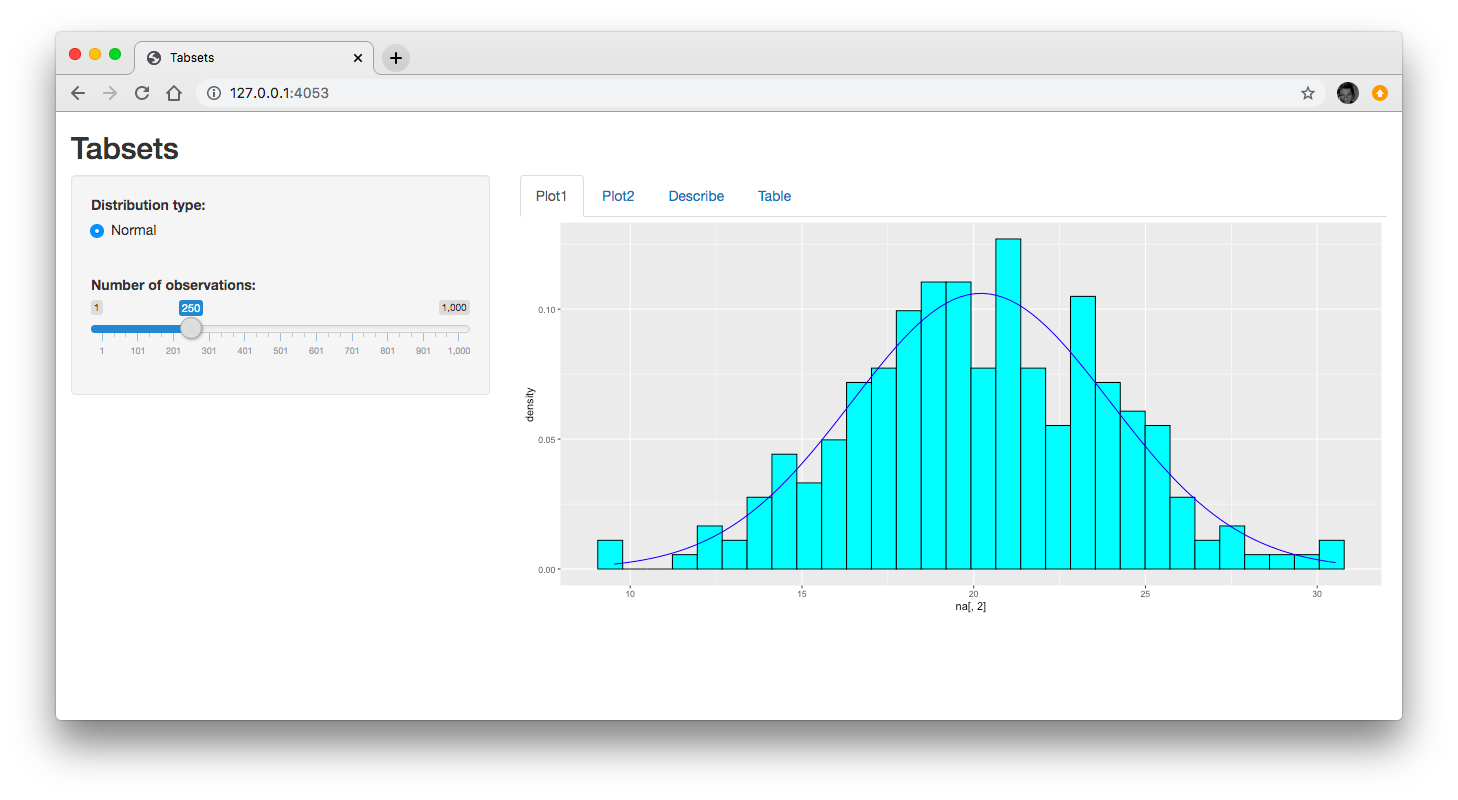
\includegraphics{./img/Shiny-Example.png}
\caption{Shiny Beispiel}
\end{figure}

\url{https://katsuckow.shinyapps.io/shiny/}

Link zu einer App, die die Normalverteilung von Daten in einem Histogram
und q-q Plot darstellt. Ausserdem werden noch verschiedene statistische
Eckdaten der Verteilung und die jeweiligen dargestellten Werte
aufgelistet. Auf dem Slider auf der linken Seite kann man die Anzahl der
übergebenen Werte ändern. Man kann daran sehen, wie die Verteilung bei
ansteigender Anzahl von Werten zunehmend einer Normalverteilung ähnelt.

\bibliography{book.bib,packages.bib}

\end{document}
